\section{BAR graph hardware}
To save I/O pins or in the case that more I/Os are needed then available often daisy chained shift registers are used. With shift registers only three microcontroller I/O pins are needed to create n*8 port I/Os. In our case we need 40 digital outputs to power the 40 leds of the led bar graph. This is realized using five 8-bit shift registers. The SN74HC595 8-bit shift registers are used which have 3-state buffer outputs. The SN74HC595 also functions as a output driver for the bar graph leds.

\begin{figure}[H]
   \centering
   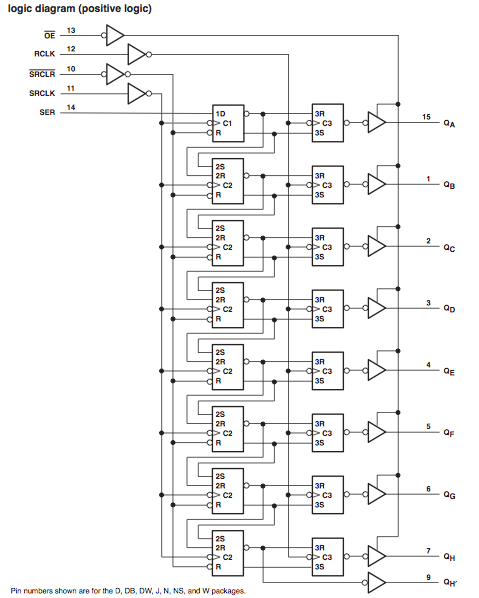
\includegraphics[width=0.5\textwidth]{img/Shift_register.png}%
   \caption{Shift register, source \url{http://www.ti.com/lit/ds/symlink/cd74hc595.pdf}}
   \label{fig:shiftRegister}%
\end{figure}


\begin{figure}[H]
   \centering
   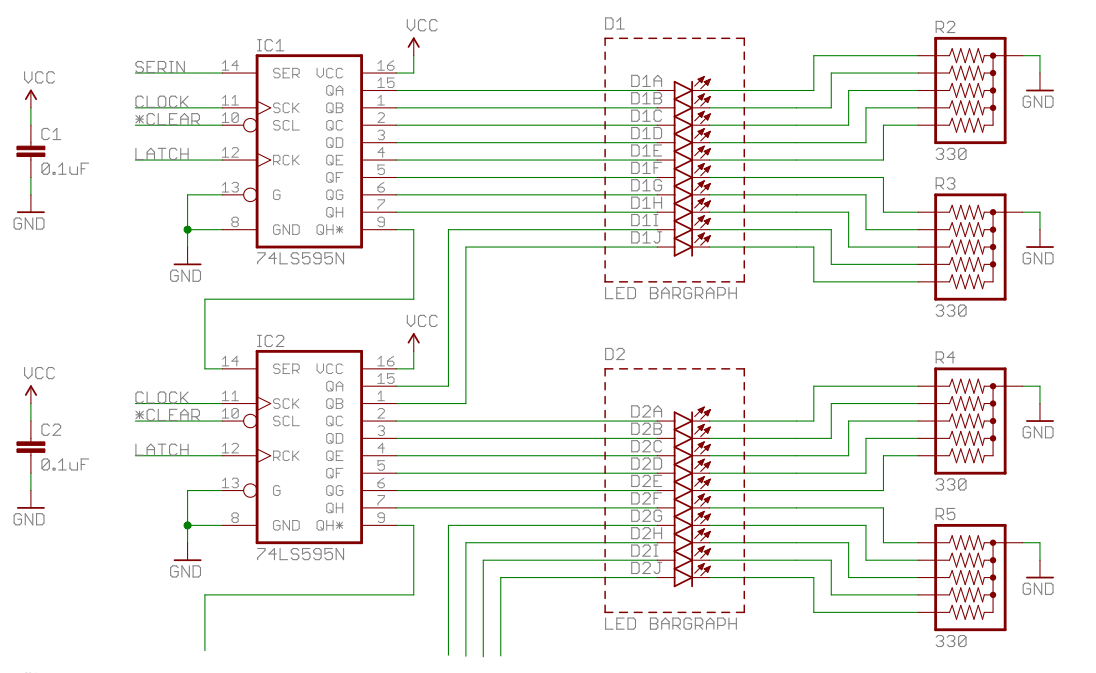
\includegraphics[width=0.8\textwidth]{img/Breakout.png}%
   \caption{Source \url{http://dlnmh9ip6v2uc.cloudfront.net/datasheets/BreakoutBoards/Bargraph Breakout v10.pdf}}
   \label{fig:breakout}%
\end{figure}

\section{Panda Board I/O - Level conversion}
The PandaBoard has two pin headers (J3 and J6) for external peripherals. Each connector has 28 pins.
Since we need a synchronous serial data stream for the shift registers we can utilize the SPI interface of the external I/O pin headers. For the required latch signal is generated with a free GPIO pin. 
In our case we use the SPI interface and the GPIO pin 140 from the PandaBoards external I/O pin header J3.


\begin{figure}[H]
   \centering
   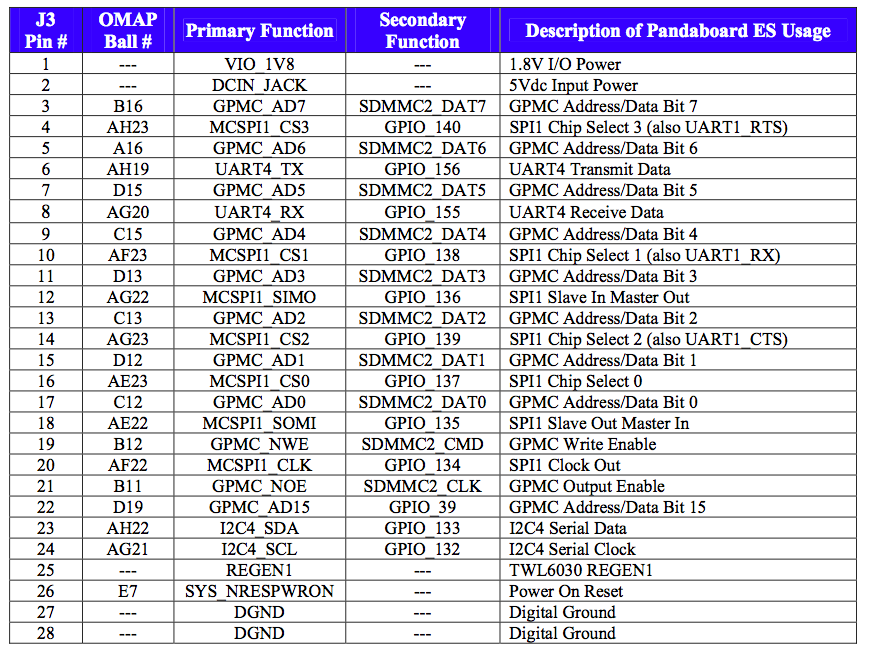
\includegraphics[width=0.8\textwidth]{img/PandaBoard_IO_J3.png}%
   \caption{Pandaboard IO J3 connectors,  source  \url{http://pandaboard.org/sites/default/files/board_reference/ES/Panda_Board_Spec_DOC-21054_REV0_1.pdf}}
   \label{fig:pandaBoardIOJ3}%
\end{figure}


\begin{table}[H]
\centering
\begin{tabular}{| l |  p{7cm} |}
\hline
\textbf{Pin} & \textbf{Used for} \\ \hline
1 & 1.8 volt reference for the level shifter. \\ \hline
2 & 5 volt for shift register, LEDs and level shifter. \\ \hline
4 & GPIO 140 for the latch signal. \\ \hline
12 & SPI 1 slave in master out  for serial data stream. \\ \hline
20 & SPI 1 clock for shift register clock signal. \\ \hline
27 & GND \\ \hline
28 & GND \\
\hline
\end{tabular}
\caption{Used J3 pins for this project}
\label{tab:pinUsageTable}
\end{table}

The PandaBoard is based on the Texas Instruments OMAP 4 application processor. The digital I/Os of the OMAP are 1.8 volts based. On the other hand the led bar graph circuit is designed using TTL levels.   
For the signal level adaptation from 1.8 volt to 5 volt a level shifter of the  74LVC8T245 type is being used. 

\begin{figure}[H]
   \centering
   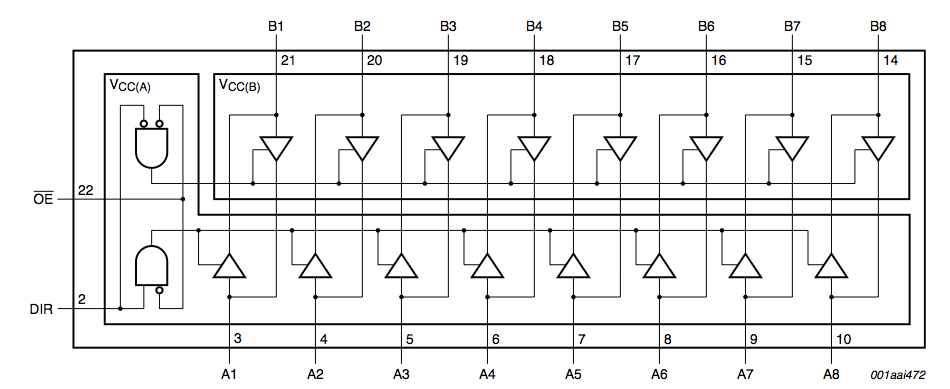
\includegraphics[width=0.8\textwidth]{img/level_Shifter.png}%
   \caption{Level shifter, source NXP  74LVC8T245 Manual}
   \label{fig:level_Shifter}%
\end{figure}

\begin{figure}[H]
   \centering
   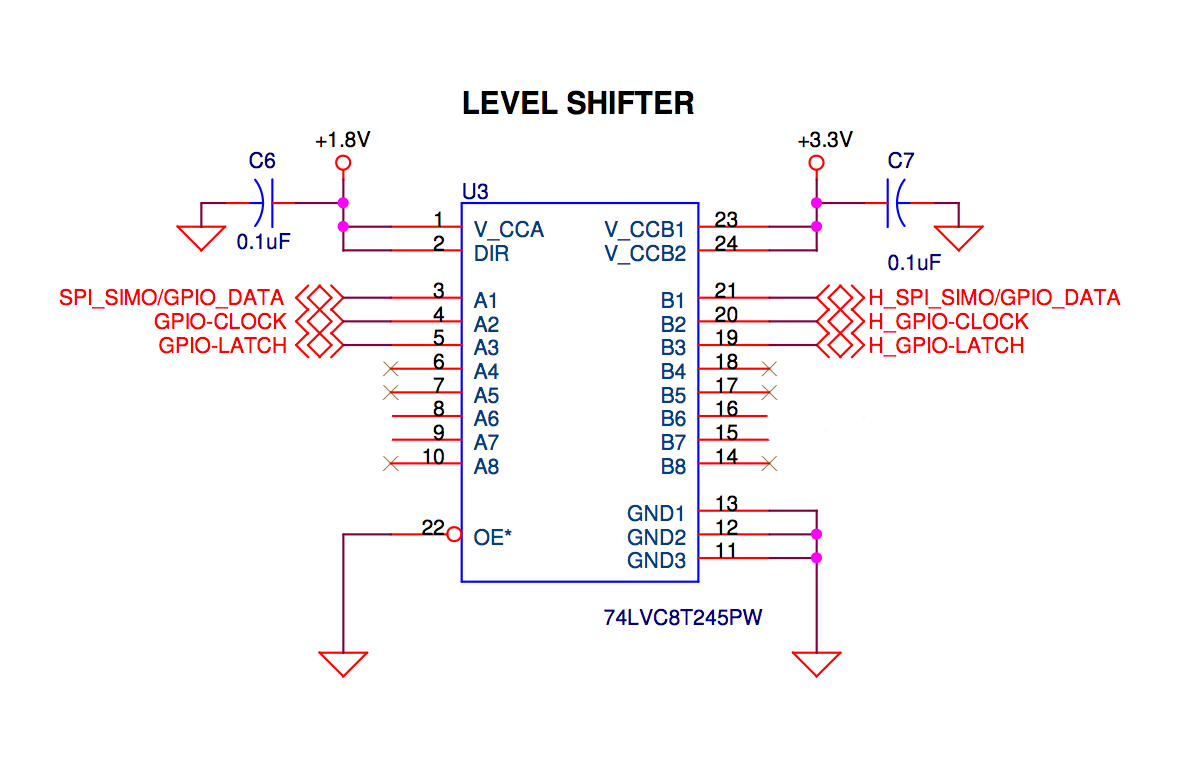
\includegraphics[width=0.8\textwidth]{img/Levelshifter.png}%
   \caption{Shift register picture, source: \url{http://www.tincantools.com/assets/BEACON REV-B .pdf}}
   \label{fig:levelShifter2}%
\end{figure}